%%%
%%%  VFlib 3.5.0 document 
%%%  Revised: 1 September 1998 
%%%
%%%  VFlib 3.5.0 --- a general font library that supports multiple font formats
%%% 
%%%  by Hirotsugu Kakugawa
%%%
%%%  Email: h.kakugawa@computer.org
%%%  FAX:   +81-824-24-0757
%%%
%%%  Research Institute for Information Science and Education
%%%  Hiroshima University
%%%  1-7-1 Kagamiyama, Higashi Hiroshima, Hiroshima,
%%%  739-8521 JAPAN
%%%

\documentclass{cah-gut}
\usepackage{graphicx}
\usepackage{shortvrb}
\usepackage{english}
\usepackage{germanb}

\newcommand{\pkg}[1]{\textsf{#1}}
\newcommand{\prog}[1]{\texttt{#1}}
\newcommand{\file}[1]{\texttt{#1}}
\newcommand{\var}[1]{\textit{#1}}
\newcommand{\VFlib}{\pkg{VFlib}}
\newcommand{\freetype}{\pkg{FreeType}}
\newcommand{\tlib}{\pkg{T1Lib}}
\newcommand{\vflibcap}{\pkg{vflibcap}}
\newcommand{\hbfgf}{\prog{hbf2gf}}
\newcommand{\ttfpk}{\prog{ttf2pk}}
\MakeShortVerb{\|}

%%%---

\setcounter{page}{1}
\NoC{0}
\DateC{}

%%%----

\begin{document}
\selectlanguage{american}

%%%-----------------------------------------------------------------------

\title{VFlib 3.5.0 --- a general font library that
       supports multiple font formats\footnote{
          This paper is based on 
          ``VFlib --- a general font library that
             supports multiple font formats,'' by Hirotsugu Kakugawa,
           Euro\TeX 98, Saint-Malo, France, 1998.}
       }
\author{Hirotsugu Kakugawa}
\affiliation{%
   Research Institute for Information Science and Education\\
   Hiroshima University\\
   1-7-1 Kagamiyama, Higashi Hiroshima, Hiroshima,\\
   739-8521 JAPAN}
\authorhead{Hirotsugu Kakugawa}
\titlehead{A font library VFlib 3.5.0}
\maketitle


%%%-----------------------------------------------------------------------

\begin{Abstract}
  \VFlib\ is a font library written in C providing several functions
  to obtain bitmaps of characters (i.e., a rasterizer).
  \VFlib\ hides the font format of font files and provides a unified API 
  for all supported font formats.  
  Thus, programmers of application software need not worry
  about font file formats and  any software using \VFlib\ 
  can support various font file formats immediately.  In addition to
  this, when a new font format is supported by \VFlib, application
  software need not be modified to use such new fonts.
  
  \VFlib\ has been developed for not only Latin fonts but also Asian
  scripts such as Chinese, Japanese, and Korean.  Since it is designed
  as a general font module, it can be used in DVI drivers for \TeX\ 
  and \LaTeX.   In this paper, we explain the API of \VFlib, a font 
  database file called \vflibcap, and the internal structure of \VFlib.
\end{Abstract}


%%%-----------------------------------------------------------------------

\begin{Keywords}
  digital fonts, computer typography, multilingual typography, 
  multilingual information processing, \TeX
\end{Keywords}


%%%-----------------------------------------------------------------------

\section{Introduction}
\label{SEC:Introduction}

Commercially and freely available fonts exist in many
different font file formats.  When we develop software to display or
print characters which do not depend on a particular window system 
and/or an operating system, we must write interface routines for 
accessing font files for each application program again and again.  
To do this, programmers must have knowledge of font file formats; 
it will be a difficult task for programmers if the number of font 
formats that an application program supports becomes large.

\VFlib\ is a font library written in C providing several functions to
obtain glyphs (bitmaps).  \VFlib\ hides the font format of font
files and provides a unified API for all supported font formats so
that programmers for application software need not worry about
font file formats.  Thus, any software using \VFlib\ can support
various font file formats immediately without modification even when
\VFlib\ is updated to support new font file formats.  
Furthermore, \VFlib\ is not window- or operating-system dependent. 

As far as the author knows, there is no general font library other than
\VFlib\ that supports multiple font formats in a platform-independent
way and that provides a unified API for font access.
For example, X~Window servers support multiple font formats.
But to use a font service, an X server process is required.  
Some font libraries have been proposed for general use: 
\freetype\ 1.1 by David Turner, Robert Wilhelm, and Werner Lemberg is a 
library for accessing TrueType fonts \cite{FreeType}. 
The \tlib\ by Rainer Menzner is a library to handle
Type~1 PostScript fonts \cite{TypeOneLib}.  
Although both are very useful libraries not dependent on 
window or operating systems, each of them supports only one 
font format and has a different API.

Conversion of font formats so that application software can use 
multiple font formats is one possible approach.  For example,
\ttfpk\ \cite{TTFTOPK} (TrueType fonts to PK fonts) 
and \hbfgf\ \cite{HBFTOGF} (HBF\footnote{
    The Hanzi Bitmap Font (HBF) format \cite{HBFspecs} 
    is a binary format for bitmap fonts for 
    Japanese, Chinese, and Korean characters.
}
fonts to GF fonts), 
both written by Werner Lemberg, makes these font formats 
available to \TeX. This method is useful but one drawback 
is that we must convert many font files in advance.

Currently, \VFlib\ supports the following font file formats: 
PCF, BDF, HBF, TrueType, Type~1, GF, PK, TFM, VF, Syotai Kurabu 
and JG \footnote{
    PCF (Portable Compiled Font) format is a binary format 
    for bitmap fonts used on X-Window.
    BDF (Bitmap Distribution Format) \cite{BDFSpec} 
    is an ASCII format for distributing binary fonts.
    Syotai Kurabu, which means \textit{font club} in English,
    is a vector font format for Japanese Kanji characters.
    JG format is another vector font format for
    Japanese Kanji characters.
}.  
To search \TeX\ font files (e.g., PK, GF, TFM, VF files)
and TrueType font files, 
\VFlib\ uses the \pkg{kpathsea} library 3.2 by Karl Berry \cite{Kpathsea}.  
\VFlib\ can be used as a font module for
drivers and previewers of DVI files generated by \TeX\ and \LaTeX.

This paper describes \VFlib\ version 3.5.0\footnote{
    \VFlib\ version 3.2 is introduced in \cite{Werner97} and
    version 3.3 is reported in \cite{Kakugawa98a}.
}.  
\VFlib\ versions 1 and 2 were designed and implemented 
for Japanese fonts only; they are widely used
in many localized software packages in Japan, 
e.g. by \pkg{Ghostscript}, \pkg{dvi2ps}, and \pkg{xdvi} 
for printing Japanese Kanji characters.  
\VFlib\ version 3 is designed for multilingual
document processing in English, French, Chinese, Japanese,
Korean, and other languages.

This paper is organized as follows.  In section \ref{SEC:ConceptsOfVFlib}, 
the basic concepts of \VFlib\ are explained.
The API of \VFlib\ is shown in section \ref{SEC:VFlibOfAPI}, and the
font database called \vflibcap\ is explained in section
\ref{SEC:Vflibcap}.  An interesting feature of \VFlib\ is the
ability to provide fonts without font files.  Section
\ref{SEC:ClassesWithoutFontFiles} explains this feature.  The author
has developed several sample programs using \VFlib, and one of these is
introduced briefly in section \ref{SEC:SamplePrograms}.  
Section \ref{SEC:Conclusion} gives concluding remarks.


%%%-----------------------------------------------------------------------

\section{Basic Concepts}
\label{SEC:ConceptsOfVFlib}

\subsection{System components}

The \VFlib\ system consists of two parts:

\begin{enumerate}
\item A library (\file{libVFlib.a}) \\
  It provides several C functions.  Any application software using
  \VFlib\ must link with this library.
\item A font database file (\file{vflibcap}) \\
  This file defines fonts and their properties (called {\em capabilities}),
  such as point size and the font file format.  Its syntax is lisp-like
  notation.
\end{enumerate}

When we initialize \VFlib, we can specify a \vflibcap\ file to be used
and thus different font sets can be used by different software.

\subsection{Font classes and font drivers}

\VFlib\ can handle multiple font file formats.  Reading a font file
according to the font file format is done by an internal module in
\VFlib\ corresponding to its font file format.  This internal module
is called a {\em font driver}.  Service units provided by font drivers
are called {\em font classes}.  From an end-user's point of view,
various font formats are distinguished by various names of font
classes.  Font drivers are internal to \VFlib\ and invisible to
end-users.

Some font drivers may not read font files on disk: they may generate
glyphs and outlines by internal computation only.  In addition, some
font drivers may return glyphs which are obtained as glyphs by another
font class.

\subsection{A view of \VFlib\ font from end-users perspective}

Each (virtual) font by \VFlib\ has its inherent information of point
size, pixel size, and resolution of the target device.  In addition,
font metrics are defined for each glyph.  
Some font file formats may not have such concepts.
For instance, TrueType font files are vector font
files and do not have information on point size.  
Syotai Kurabu format fonts do not have font metric information at all.  
In such case, either (1)~the lacking information 
is given in \vflibcap\ or (2)~the specific font driver gives such 
information as default values. 

\subsection{Font names and font searching mechanism}

In \VFlib, a font is specified by a {\em font name} on opening.
First, \VFlib\ checks whether the font name is given in \vflibcap\ or
not.  If the font name is found, \VFlib\ reads the description for the
font in \vflibcap.  The description contains a font class name; \VFlib\ 
then invokes a font driver corresponding to the font class name.
Finally the font driver opens the font file (if necessary).

If the font name is not given in a \vflibcap\ file, a font searching
mechanism is invoked.  Since there are many font files for X~Window
and \TeX, this feature is introduced to avoid writing an entry for
each font file.  Various font drivers will be called to see whether
the font can be opened; a list of font drivers for font searching is
given in the \vflibcap\ file.  If a font driver succeeds in opening the
font, font searching finishes and the \VFlib\ font opening function
returns successfully.  Otherwise, font open fails.

Fonts described in a \vflibcap\ file are called {\em explicit fonts} and
fonts that are searched for by the font search feature are called {\em
  implicit fonts}.

\subsection{Two modes of opened fonts}

The following two modes are provided to obtain glyphs of fonts.
\begin{itemize}
\item High resolution device-oriented mode (mode 1)\\
  The size of glyphs is specified by the physical size of
  glyphs and device resolution. 
\item Low resolution device-oriented mode (mode 2)\\
  Glyph sizes are specified by pixel size rather than by
  device resolution.  
\end{itemize}
When the size of a glyph in the
source font is different from the target size, \VFlib\ scales the
source glyph internally.
Thus, users need not know know original size of glyphs in font files.

Two modes are provided by the following reason.
When we write a application programs that prints documents on printer, 
it is convenient to specify glyph size by point and device resolution
such as glyph of 12 point for a 300 dpi printer.
On the other hand, when we write a application programs 
that displays documents on CRT screen,
it is convenient to specify glyph size by pixel.

\subsection{Internal Structure}

The \VFlib\ library consists of a {\em core} and several {\em font
  drivers}.  The \VFlib\ core provides entry functions of the API, 
as well as a font driver table, opened font table, \vflibcap\ access module,
and other utility modules.  The internal structure of \VFlib\ is
depicted in Figure \ref{FIG:VFlibInternal}.

\begin{figure}
  \begin{center}
    \mbox{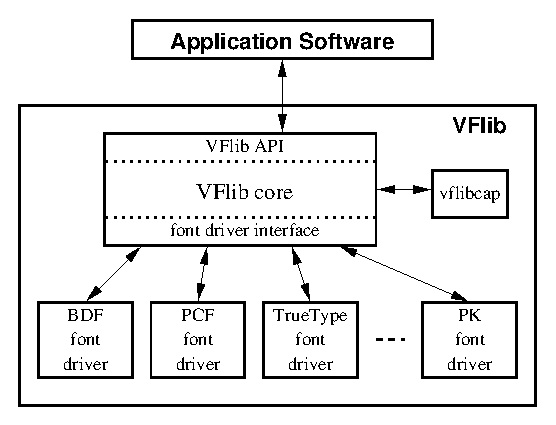
\includegraphics[scale=1.0]{internal.eps}}
  \end{center}
  \caption{Internal structure of \VFlib}
  \label{FIG:VFlibInternal}
\end{figure}

Each font driver has corresponding functions for each font operation
of \VFlib.  Such functions are implemented to provide \VFlib\ 
API-compatible behaviour.  
The set of capabilities that can be used for each font class 
in \vflibcap\ file may differ; each font class defines 
the capabilities it needs.


%%%-----------------------------------------------------------------------

\section{The API}
\label{SEC:VFlibOfAPI}

In this section we describe the API of \VFlib.  The API that \VFlib\ 
defines is simple.  For example, as a contrast, \freetype\ defines 
a rich set of functions including access to kerning information.  
The simplicity of \VFlib\ API is a result of the limitation that 
it must be common to every font format that \VFlib\ supports.  
\VFlib\ does not have features for typesetting such as obtaining 
kerning information of fonts.  But it is enough strong to print and 
display typesetted documents such as DVI files.

\subsection{Data types}

\VFlib\ defines the following three data types for font access: bitmaps
and metrics for modes~1 and~2.

\begin{itemize}  
\item Bitmap object \\
  A bitmap object is a set of font metrics and bitmap data.  The
  following is the definition of bitmap structure.

\begin{quote}
\begin{small}
\setlength{\baselineskip}{1em}
\begin{verbatim}
struct vf_s_bitmap {
  int             bbx_width, bbx_height; /* in pixels */
  int             off_x, off_y;          /* in pixels */
  int             mv_x,  mv_y;           /* in pixels */
  unsigned char*  bitmap;
  int             raster;
};
\end{verbatim}
\end{small}
\end{quote}

  The members \prog{bbx\_width} and \prog{bbx\_height} are the width
  and height of the bitmap, respectively.  The members \prog{bitmap}
  and \prog{raster} are pointers to the glyph data and the number of
  bytes of a raster.  The members \prog{off\_x} and \prog{off\_y} 
  form a vector from the reference point to the upper-left corner of a
  bitmap.  The members \prog{mv\_x} and \prog{mv\_y} form a vector to
  the next reference point.  Metric information is given in pixel form.
  
\item Metric object (modes 1 and 2) \\
  Metric objects for modes~1 (high resolution device-oriented mode)
  and~2 (low resolution device-oriented mode) are defined similarly 
  as bitmap objects except that they do not have \prog{bitmap} and
  \prog{raster} members.  Member types of mode~1 metric objects 
  are \prog{double}, not \prog{int}; their units are points rather 
  than pixels.
\end{itemize}

\subsection{Functions}

\begin{itemize}
\item \prog{int VF\_Init(char* \var{vflibcap},
                         char* \var{variable\_list})} \\
  Initialize \VFlib.  The first argument \var{vflibcap} is the file name
  of a \vflibcap\ file.  The second argument {\it variable\_list} is a 
  list of parameters passed to \VFlib\ for parameterization of \vflibcap.
  (See subsection \ref{SUBSEC:VFLIBCAP:PARAM} for details of
  parameterization.)

\item \prog{int  VF\_OpenFont1(char* \var{font\_name},
                               double \var{dpi\_x},
                               double \var{dpi\_y}, 
                               double \var{point\_size}, 
                               double \var{mag\_x},
                               double \var{mag\_y})} \\
  Open a font in mode~1.  The font name is given by the first
  argument.  Two arguments \var{mag\_x} and \var{mag\_y} are
  horizontal and vertical magnification factors.  The actual font size
  is determined by these arguments.  This function returns a font
  identifier (font id) for the opened font.  All font operations take
  this font id to specify a target font.

\item \prog{int VF\_OpenFont2(char *\var{font\_name},
                              int \var{pixel\_size},  
                              double \var{mag\_x}, 
                              double \var{mag\_y})} \\
  Open a font in low resolution mode.  This function is similar to
  \prog{VF\_OpenFont1()} except font size is given in pixels.

\item \prog{VF\_BITMAP  VF\_GetBitmap1(int \var{font\_id}, 
                                       long \var{code\_point},
                                       double \var{mag\_x}, 
                                       double \var{mag\_y})} \\
  Obtain a glyph bitmap of a given font id (in mode~1) and code point.
  The font id \var{font\_id} must be an id returned by
  \prog{VF\_OpenFont1()}.  The size of the bitmap to be obtained can
  be specified by the \var{mag\_x}, and \var{mag\_y} arguments.  

\item \prog{VF\_BITMAP  VF\_GetBitmap2(int \var{font\_id}, 
                                       long \var{code\_point},
                                       double \var{mag\_x},
                                       double \var{mag\_y})} \\
  Obtain a glyph bitmap of a given font (in mode~2) and code point.
\end{itemize}

\VFlib\ defines other functions such as \prog{VF\_""METRIC1
  VF\_""Get""Metric1()} and \prog{VF\_""METRIC2 VF\_""Get""Metric2()}
to obtain font metrics of a character of mode~1 and~2 fonts,
respectively; \prog{VF\_""OUTLINE VF\_""Get""Outline()} to obtain
\VFlib\ format vector data of a character of mode~1 fonts; and
\prog{VF\_""BITMAP VF\_""Outline""To""Bitmap()} to convert \VFlib\ format
vector data to a bitmap.  By calling
\prog{VF\_""Install""Font""Driver()}, a font driver is installed.


%%%-----------------------------------------------------------------------

\section{A Font Database File ``\vflibcap''}
\label{SEC:Vflibcap}

A \vflibcap\ file is a database of font definitions for \VFlib.  It is
read when \VFlib\ is initialized.  A simple example of a \vflibcap\ file
is shown below:

\begin{quote}
\begin{small}
\setlength{\baselineskip}{1em}
\begin{verbatim}
(define-default  VFlib
  (uncompression-programs  (".Z" "zcat") (".gz" "gzip -cd"))
  (implicit-font-classes  pcf bdf)
  (extension-hints  (".bdf" bdf) (".pcf" pcf)))

(define-default  bdf
  (filename-extensions ".bdf")
  (font-directories  "/usr/local/share/fonts/X11//")
  (compression-extensions ".gz" ".Z"))

(define-default  pcf
  (filename-extensions ".pcf")
  (font-directories  "/usr/X11R6/lib/X11/fonts//"
                     "/usr/openwin/lib/X11/fonts//")
  (compression-extensions ".gz" ".Z"))

(define-font  timR24    ; Times Roman 24pt, BDF format
  (font-class bdf)
  (dpi 300) (point-size 24)
  (font-file "timR24.bdf"))

(define-font  timR18    ; Times Roman 18pt, PCF format
  (font-class pcf)
  (dpi 300) (point-size 24)
  (font-file "timR18.pcf"))
\end{verbatim}
\end{small}
\end{quote}

By a \prog{define-default} construct, a default values of a font class
is defined.  By a \prog{define-font} construct, a font is defined.  
Semicolon (\prog{;}) starts a comment.
In this example, there are three definitions for font class default
(\prog{VFlib}, \prog{BDF}, and \prog{PCF}) and two font definitions
(\prog{timR24} and \prog{timR18}). The first three entries are used to
give default parameters for \VFlib\ and each font class.  We explain
these entries later and explain the other two entries first.  Although
many capabilities are defined, we explain only the fundamental ones.

\subsection{Font entries}

The entry \prog{timR24} has several capabilities.  A capability
\prog{font-""class} specifies the font class name.  In this example,
\prog{timR24} belongs to the \prog{bdf} font class.  
The capabilities \prog{dpi} and \prog{point-""size} give 
device resolution and point size of a font.
These values are used when this font is opened in mode~1.  
A capability \prog{pixel-""size} gives the pixel size.  
This value is used when this font is opened in mode~2. 
The capabilities \prog{pixel-""size}, \prog{dpi}, and \prog{point-""size}
can be omitted since a BDF font file contains their values.  
A capability \prog{font-""file} gives the file name of the font.
Similarly, \prog{timR18} is defined except in cases of PCF fonts.

The two font files \prog{timR24.bdf} and \prog{timR18.pcf} are both
bitmap fonts used in X~Window.  Although pixel size, point size, and
target device resolution are together with the bitmap given in the
font file, \VFlib\ internally enlarges or shrinks bitmaps to yield the
requested size.  From a user's point of view, only the font names
(\prog{timR24} and \prog{timR18}) are visible; users need not be aware
of font formats.

\subsection{Default descriptions}

In the example above, there are three default descriptions.  The first
entry \prog{VFlib} is used to give global parameters of \VFlib.  In
our example, the relation between the filename extension and an
uncompression program is given by the capability
\prog{uncompression-""programs}; it specifies that files whose names
end in \prog{.Z} and \prog{.gz} are uncompressed by running commands
\prog{zcat} and \prog{gzip -cd}, respectively. 
The capability \prog{implicit-""font-""classes} specifies a
list of font classes that search implicit fonts.  When a font is
opened and a corresponding entry is missing in \vflibcap, font drivers
given by this capability are called to search the font in given order.
Suppose a font named \prog{timR10.bdf} is requested to open.  Since
such an entry does not exist in the \vflibcap\ file, the font is
searched as an implicit font by calling the PCF font driver first, and
then the BDF font driver.  A capability \prog{extension-""hints} gives
a relation of font name extension and font class.  In the example, if
an extension of a font name is \prog{.pcf} (\prog{.bdf}), the PCF
(BDF) font driver is called for implicit font search.  For example, if
a font named \prog{timR08.bdf} is requested to open, the BDF font
driver is called.  This is useful for searching implicit fonts fast.

The next definition \prog{BDF} is a default description for the BDF
font class.  A capability \prog{font-""directories} is a list of font
directories in which font files are stored.  If the directory name is
terminated by \prog{//}, files are searched recursively under the
directory.  The entry \prog{compression-""extensions} gives a list of
file compressions that BDF font class supports.
Similarly, default definition for \prog{PCF} font class is given.

\subsection{Parameterized \vflibcap}
\label{SUBSEC:VFLIBCAP:PARAM}

Capability values in \vflibcap\ can be overridden at execution time.
By this feature, called {\em parameterization}, several applications 
can share the same \vflibcap\ file.
The next example is a \vflibcap\ for printer driver for \TeX\ DVI file
for 300 dpi Canon Laser Shot.
Note that all fonts are implicit fonts.

\begin{quote}
\begin{small}\setlength{\baselineskip}{1em}
\begin{verbatim}
(define-default  VFlib
  (implicit-font-classes  pk)
  (extension-hints  ("pk" pk))
  (variable-values  (TeX_USE_KPATHSEA      "Yes")
                    (TeX_DPI               "300")
                    (TeX_KPATHSEA_MODE     "cx")
                    (TeX_KPATHSEA_PROGRAM  "/usr/local/bin/xldvi"))
  (use-kpathsea           $TeX_USE_KPATHSEA)
  (kpathsea-mode          $TeX_KPATHSEA_MODE)
  (kpathsea-program-name  $TeX_KPATHSEA_PROGRAM) )

(define-default  TeX
  (dpi $TeX_DPI)
  (tfm-directories  "TEXMF" "/usr/local/fonts/tfm")
  (tfm-filename-extensions  ".tfm"))

(define-default pk
  (font-directories  "TEXMF" "/usr/local/fonts/pk"))
\end{verbatim}
\end{small}
\end{quote}

In the \prog{VFlib} entry, the capability \prog{variables-""values}
gives a list of variable names and their default values.  In this
example, there are three variables. For instance, the default value of
\prog{TeX\_""DPI} is \prog{300}.  A capability value can be a value of
a variable if a dollar sign (\prog{\$}) followed by a variable name is given.  
In the \prog{VFlib} entry, initialization parameters for \pkg{kpathsea}
are given.

In the \prog{TeX} entry, which is used to specify a common 
default description  for \TeX\ related font classes, 
the value of the capability \prog{dpi} 
is given as the value of a variable \prog{TeX\_""DPI}, for example.
Capabilities \prog{tfm-directories} is a list of TFM files directories, 
and \prog{tfm-""filename-""extensions} is a extension of a file name 
for TFM files.
The name \prog{"TEXMF"} in \prog{tfm-""directories} is a special name 
to seach a file using \pkg{kpathsea}.

The entry \prog{pk} entry is used to specify default description 
for font files in PK format.
A PK file is search by \pkg{kpathsea} first since the first item
of the value of the capability \prog{font-""directories} is \prog{"TEXMF"}.
If it is not found, then it is searched in \prog{/usr/""local/""fonts/pk}
directory next.

Default variable values can be overridden by giving a list of pairs of
variable names and their values when \VFlib\ is initialized by
\prog{VF\_Init()}. If a Unix environment variable
\prog{VFLIBCAP\_""PARAM\_\var{var}} (e.g.,
\prog{VFLIBCAP\_""PARAM\_TeX\_DPI} is defined, its value becomes the
value of the \vflibcap\ variable \prog{TeX\_""DPI}.)
The example \vflibcap\ file can be used for 600 dpi HP Laser Jet 4 printers 
if we override variable values so that
\prog{TeX\_""DPI} is \prog{600} and \prog{TeX\_""KPATHSEA\_""MODE} is
\prog{ljfour} on execution time without any file modification.


%%%-----------------------------------------------------------------------

\section{Font Classes without Font Files}
\label{SEC:ClassesWithoutFontFiles}

\begin{figure}
\begin{center}
\mbox{
\includegraphics[scale=0.75]{comic-jp.eps}}
\end{center}
\caption{Mixture of {\it gothic} and {\it mincho} fonts in Japanese comics}
\label{FIG:JpComics}
\end{figure}

Fonts provided by font classes need not be associated with font files.
As examples of such font classes, 
the {\em Japanese comic} font class and
the {\em try} font class are implemented.

\subsection{The Japanese comic font class}

In Japanese comics, a gothic font is used for Kanji
characters and a {\it mincho} font is used for Kana
characters as shown in Figure \ref{FIG:JpComics}.  
Without creating a new font, we can implement such fonts by 
the  Japanese comic font driver: 
a font $F$ of the Japanese comic class needs two sub-fonts that are
specified in a \vflibcap\ file; fonts for Kanji characters, say $F_1$,
and Kana characters, say $F_2$.  
A glyph for code point $c$ of font $F$ is obtained from $F_1$ if $c$ 
is a Kanji character, and from $F_2$ if $c$ is a Kana character.  
The font classes of $F_1$ and $F_2$ need not be the same.


\subsection{The try font class}

The try font class provides a feature to open a font among list of fonts.
Each font $f$ of the try font class has a list of fonts, say $g_1, g_2, ...$.
When $f$ is requested to open, the font driver tries to open fonts
$g_1, g_2, ...$ in this order until one of them, 
say $g_s$, is opened successfully.
Then, any font operation on $f$ is applied on $g_s$ and 
therefore, $g_s$ is used as a font $f$.

This font class is useful when we want to use non-standard 
(i.e., site dependent) fonts.
Suppose that a non-standard font $f_n$ is listed followed by
a standard font $f_s$ in a font list of $f$ of try font class.
Then, to open $f$ is the same as opening $f_n$ if it is avaiable; 
otherwise, $f_s$ is used.
Since $f_s$ is a standard font, opening $f$ always succeeds.
Candidate fonts $g_1, g_2, ...$ can be a fonts of different font classes;
for instance, $g_1$ can be a TrueType font and $g_2$ can be a PCF font. 



%%%-----------------------------------------------------------------------

\section{Sample Programs}
\label{SEC:SamplePrograms}

\VFlib\ is distributed with sample programs.  
One of them is a previewer for DVI files.  
In a DVI interpreter, a \TeX\ font is opened
by the following sequence.

\begin{figure}
\begin{center}
%\mbox{\includegraphics[scale=1.2]{xmdvi-image-rgb.eps}}
%\mbox{\includegraphics[scale=1.2]{xmdvi-image-gray.eps}}
\mbox{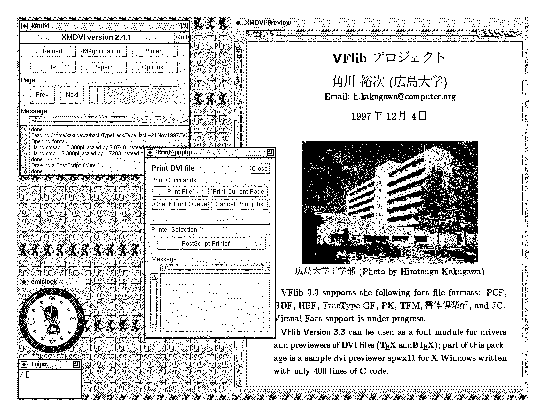
\includegraphics[scale=1.2]{xmdvi-image-bw.eps}}
\end{center}
\caption{A DVI file previewer \pkg{xmdvi}}
\label{FIG:Xmdvi}
\end{figure}

\begin{verbatim}
   sprintf(f_name, "%s.pk", name);
   fid = VF_OpenFont1(f_name, h_dpi, v_dpi, -1, mag, mag);
\end{verbatim}

The variable \prog{name} is a font name as appearing in a DVI file
(e.g., \prog{cmr10}); \prog{h\_dpi} and \prog{v\_dpi} are the
horizontal and vertical device resolution of the target device in dpi,
respectively.  The variable \prog{mag} is a magnification factor.  The
PK font driver finds an appropriate font file from parameters given in
\prog{VF\_OpenFont1()} and the default values given in \prog{TeX} 
entry in \vflibcap. For instance, if the font
name is \prog{cmr10.pk} and \prog{h\_dpi} = \prog{v\_dpi} = 300, and
\prog{mag} = 1.2, the PK font driver looks for the font file
\prog{cmr10.360pk}.  Glyphs are simply obtained by calling the
\prog{VF\_GetBitmap1()} function.

Figure \ref{FIG:Xmdvi} shows a screen shot of a sample previewer on
X~Window using Motif.  This previewer supports drawing EPS figures and
color changes.


%%%-----------------------------------------------------------------------

\section{Conclusion}
\label{SEC:Conclusion}

In this paper, we have introduced a font library \VFlib\ which
supports multiple font formats with a unified API.  
It is especially useful for DVI drivers.

\VFlib\ has been tested on 
FreeBSD 2.2.2 and Linux for Pentimun, 
Solaris 2.5.1 and SunOS 4.1.4 for SPARC, and
SunOS 4.1 for SPARC; 
there is no difficulty to port it to other Unix-like operating systems.  
The source code and the latest information on \VFlib\ 
is available at 
|http://|""|www.|""|se.|""|hiroshima-u.|""|ac.|""|jp/|"%
"|~kakugawa/|""|VFlib/|.


%%%-----------------------------------------------------------------------
\section*{Acknowledgements}
The author would like to thank Werner Lemberg for helpful comments 
on specification and implementation of \VFlib.
He also thank Ken'ich Handa and Satoru Tomura for 
valuable discussions.


%%%-----------------------------------------------------------------------

\bibliographystyle{plain}
\bibliography{vflib35}
\nocite{*}


%%%-----------------------------------------------------------------------

\end{document}

%%%EOF
